%!TEX root = ../main.tex
\chapter{Validation} % (fold)
\label{cha:validation}

\section{Presentation of the toy problems}

To demonstrate the capacities and the limitations of
the harmonic balance approach, two toy problems are set up.
The first one solves the constant convection equation within 
a harmonic balance framework, the second one is a laminar
Navier-Stokes rotating blocks configuration.

\subsection{Convection equation problem} % (fold)
\label{sub:convection_equation_problem}

The harmonic balance source term is an alternative to
a classical time marching scheme for periodic phenomenon.
The simplest unsteady equation
that can be formulated is the constant convection equation:
\begin{equation}
  \label{eq:convection}
  \frac{\partial u}{\partial t} + c \frac{\partial u}{\partial x} = 0,
\end{equation}
where $c$ denotes the constant velocity and $u$ the transported quantity.
If we impose an unsteady periodic inlet,
we obtain a simple test case for harmonic balance approach. Any kind
of input can be simulated allowing to fully investigate the properties of 
the method.

Moreover, this equation is interesting as the analytical solution is simple
and known for any input. In fact, the solution only depends on the 
initial and/or boundary conditions:
\begin{equation}
  \label{eq:solconvanalytic}
    u(x, t) = u_0(x - ct)
\end{equation}
where $u_0$ is the boundary condition. Moreover, as the equation
is simple enough, it will be easy to discriminate the effects of the
harmonic balance source term.

The convection equation is solved in a 1D cartesian mesh.
A $4$\textsuperscript{th} order centered finite
difference scheme is used to evaluate the spatial derivative:
\begin{equation}
    \left. \frac{\partial u}{\partial x} \right)_{t=q}^{x=i} \approx 
    \frac{-u^{i+2}_{q} + 8 u^{i+1}_{q} - 8 u^{i-1}_{q} + u^{i-2}_{q}}{12\Delta x},
    \label{eq:convection_center4}
\end{equation}
where $u_i^q$ is the sum of the velocity for  
all harmonic balance instants as defined in Eq.~\eqref{eq:hb_concatenation},
evaluated at position $i$ within pseudo-iteration $q$.
A $4$ step Runge-Kutta method is then use to time 
march the equation to the steady state with the coefficients $\alpha_0 = 0$,
$\alpha_1 = 1/4$, $\alpha_2 = 1/3$, $\alpha_3 = 1/2$ and $\alpha_4 = 1$.
The k\textsuperscript{th} step is evaluated by:
\begin{equation}
    u_k = u_q - \alpha_k \Delta t \left [ 
          c \left. \frac{\partial u_{k-1}}{\partial x} \right)_{t=t_q + \alpha_{k-1} \Delta t}
          + D_t(u_q)
          \right],
    \label{eq:convection_rk4}
\end{equation}
where the HB source term $D_t(u_q)$ is computed using Eq.~\eqref{eq:dt}. 

As we use 
an explicit time marching scheme, the CFL number is set to $1$ to ensure stability.
The mesh is composed of $2000$ grid points, which proved to be converged.
The period of injection is chosen so that, when the temporal frequency is
set to $1$, only one pattern 
appears at a time in the mesh
as shown in Fig.~\ref{fig:convection_injection_paper} for a Gaussian function.
This is done by setting the biggest temporal period $T$ to:
\begin{equation}
   T = \frac{L_x}{c},
\end{equation}
where $L_x$ is the size of the mesh.


As the harmonic balance computations are steady computations linked 
by a source term, 
different boundary conditions, as done in~\cite{Dufour2010},
have to be set to impose a periodic injection. Two ghost cells
are used to maintain the spatial $4$\textsuperscript{th} order scheme 
at the left
boundary condition.
\begin{figure}[htbp]
  \begin{center}
    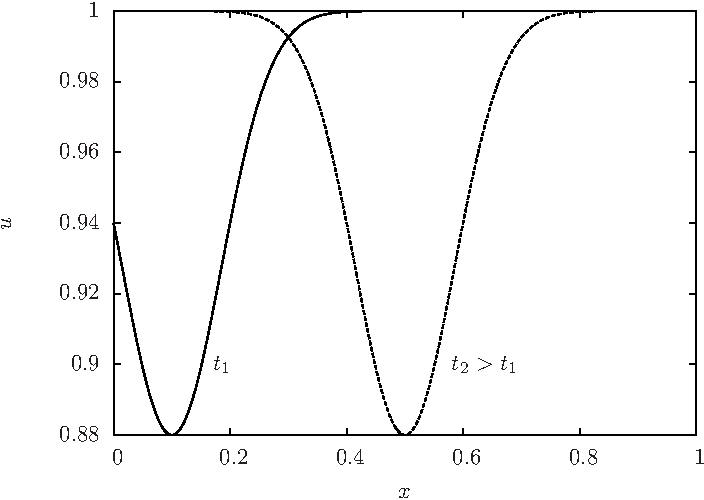
\includegraphics[width=.5\textwidth]{GAUSSIAN_INJECTION_PAPER.pdf}
  \end{center}
  \caption{Convection of the Gaussian function in the 1D cartesian mesh.}
  \label{fig:convection_injection_paper}
\end{figure}
For the right boundary condition, imposing a periodicity condition is
numerically stiff. For this reason, the scheme is degenerated 
to an upwind scheme to avoid wave reflections. The upwind scheme is degenerated to
a 2\textsuperscript{nd} order, one cell before and at first order on the 
last cell:
\begin{align}
    \left. \frac{\partial u}{\partial x} \right)_{t=q}^{x=m-1} &\approx 
    \frac{3 u^{m-1}_{q} - 4 u^{m-2}_{q} + u^{m-3}_{q}}{2\Delta x}, \\
    \left. \frac{\partial u}{\partial x} \right)_{t=q}^{x=m} &\approx 
    \frac{u^{m}_{q} - u^{m-1}_{q}}{\Delta x},
\label{eq:upwind_scheme}
\end{align}
where $m$ is the total number of grid points. This is much better than a periodicity
condition as the convected function suffers from diffusion and dispersion (even if the
mesh is small enough) that is not compatible with the injected function.

\section{Channel flow}
\label{sec:channel-flow}

\subsection{Test case description}
% presentation of the channel case
A channel configuration is set up to study the properties of the
proposed HB method and the above algorithms for non-uniform time
sampling.  It is a 2D channel of length $L_x = 100$~m in the axial
direction and $L_z = 1$~m in the transverse one.  The boundary
conditions are: (i)~an injection condition for the inlet,
(ii)~symmetric conditions for the upper and lower bounds as the flow
is assumed to be symmetric in the transverse direction, and (iii)~a
fluctuating pressure imposed at the outlet:
\begin{equation}
  P_{outlet}(t) = P_m \cdot \left[1 + A_1 \cdot \sin(2 \pi f_1 t) +
    A_2 \cdot \sin(2 \pi f_2 t) \right],
  \label{eq:outlet_canal}
\end{equation}
where $P_m$ is the temporal average static pressure, $A_n$ the
amplitude of the $n$\textsuperscript{th} mode and $f_n$ its
frequency. The mean outlet pressure $P_m$ is set to $60\%$ of the
inlet total pressure $P_{i0} = 101,325$~Pa.

Pressure waves travel within the flow with the velocity $u + c$ and $u
- c$, where $u$ denotes the local flow velocity and $c$ the sound
velocity. Since the pressure waves are generated at the outlet, only
the $u-c$ waves are visible, resulting in pressure waves propagating
upstream of the channel, which are damped by the effect of
viscosity. Figure~\ref{fig:canal_principle} shows a schematic diagram
of the channel case, illustrating the propagation and attenuation of
the pressure waves.
\begin{figure}[htb]
  \centering
  \includegraphics*[width=0.6\textwidth]{CANAL2_PRINCIPLE.pdf}
  \caption{Schematic diagram of the channel case.}
  \label{fig:canal_principle}
\end{figure}

% mesh presentation
The mesh consists of 997~points along the axial direction and 9 in the
transverse one, which amounts to almost equal spacings in both
directions.


This configuration is turbulent as the Reynolds number based on the
inlet flow velocity and the axial length of the channel is about $R_e
\approx 2.0 \times 10^9$.  Turbulence is modeled using the
one-equation model of Spalart and Allmaras~\cite{Spalart1992}, and the
third-order upwind Roe scheme~\cite{Roe1981} is used to compute the
convective fluxes.

\subsection{Convergence sensibility analysis}

As mentioned previously, the condition number is of great importance
for the convergence of the proposed HB method. To highlight this
feature, the presented channel case is computed with a single
frequency at the outlet: $f_1 = 3$~Hz with an amplitude $A_1 = 0.05$
for the first case and $A_1=0.01$ for the second one, the second
frequency having a zero amplitude: $A_2= 0$.  Two frequencies are
specified for the HB computation: $f_1$ and its first harmonic
$2f_1$. The time levels are chosen to reach varying condition numbers
such that $1 \leq \kappa (A) \leq 3.43$.  Since the input frequencies of the HB
computation are harmonically related, the minimal conditioning
$\kappa(A) = 1$ is obtained with evenly spaced time levels.  The OPT
algorithm is modified by subtracting the targeted conditioning to the
objective function, so that the different condition numbers can be
reached.  The distribution of the time levels for each condition
number is shown in Fig.~\ref{fig:canal2_distribution_tlv}.  The time
levels deviate from the evenly spaced solution as the condition number
grows.
\begin{figure}[htb]
  \centering \subfigure[Relative to period
  $1/f_1$]{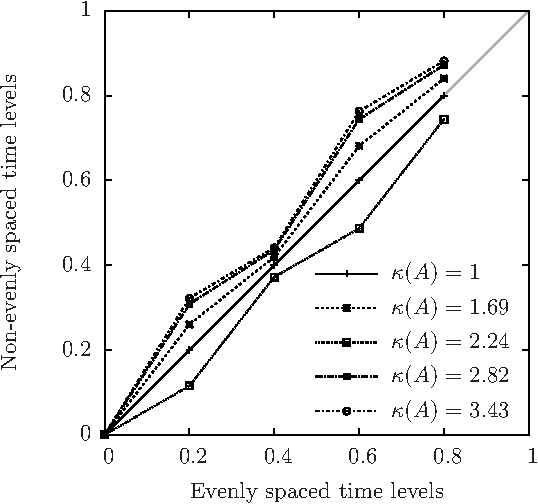
\includegraphics[width=.45\textwidth]{CANAL2_RESIDUAL_VS_CONDITIONNING_TLV_REPARTITION_F1.pdf}}
  \quad \subfigure[Relative to period
  $1/2f_1$]{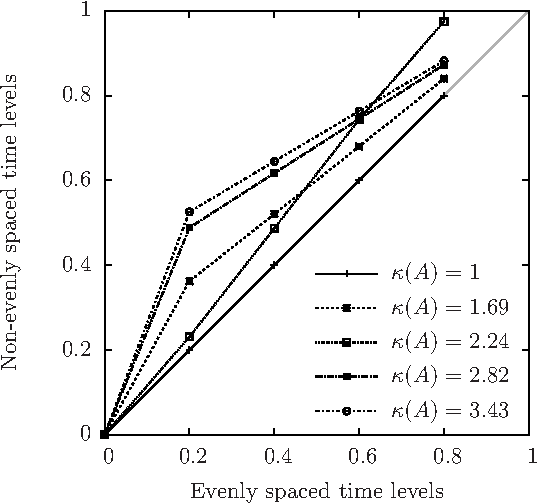
\includegraphics[width=.45\textwidth]{CANAL2_RESIDUAL_VS_CONDITIONNING_TLV_REPARTITION_F2.pdf}}
  \caption{Distribution of the time levels on each frequency periods.}
  \label{fig:canal2_distribution_tlv}
\end{figure}
The results in Fig.~\ref{fig:canal_residual_vs_conditionning} show that
for a condition number $\kappa (A) \geq 3.43$ and wave input amplitude
$A_1 = 0.05$, the computation diverges. However, the computations with
the same condition numbers but a smaller input amplitude $A_1 = 0.01$
converge. In fact, the condition number amplifies the errors made
during the iterative process. When the input waves have a smaller
amplitude, the iterative errors are slighter, hence the convergence as
explained \S~\ref{sec:condition_number}.
\begin{figure}[htb]
  \centering \subfigure[$A_1 =
  0.01$]{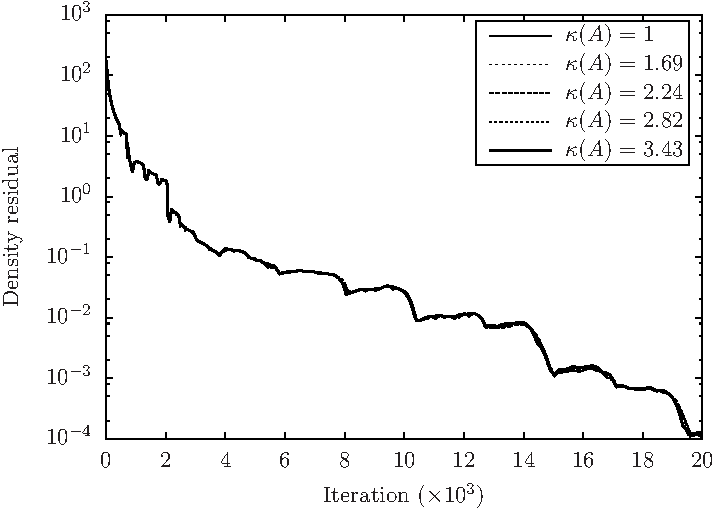
\includegraphics[width=.45\textwidth]{CANAL2_RESIDUAL_VS_CONDITIONNING_AMP001.pdf}}
  \quad
  \subfigure[$A_1=0.05$]{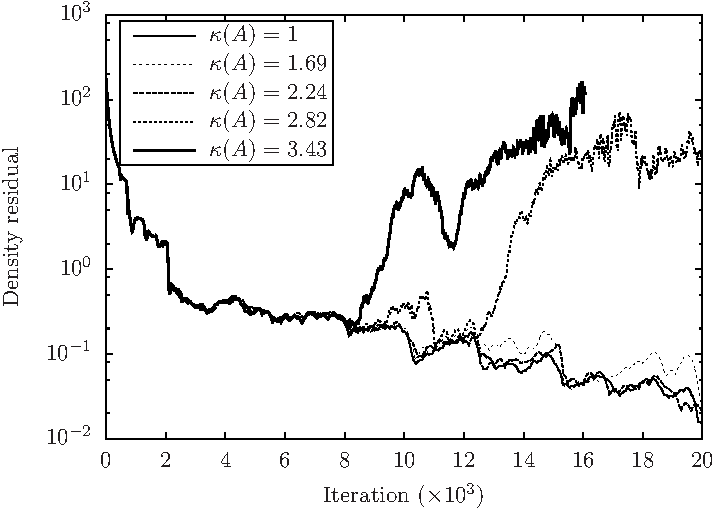
\includegraphics[width=.45\textwidth]{CANAL2_RESIDUAL_VS_CONDITIONNING_AMP005.pdf}}
  \caption{Relation between the condition number $\kappa (A)$ and the
    convergence of the solution.}
  \label{fig:canal_residual_vs_conditionning}
\end{figure}


\subsection{Validation of the multi-frequency HB method}

To validate the proposed HB method, two non-harmonically related
frequencies are chosen as input for the outlet boundary condition:
$f_1 = 3$~Hz and $f_2 = 17$~Hz.

A classical time-marching scheme is taken for comparison, namely the
Dual Time Stepping scheme (DTS~\cite{Jameson1991}).  The DTS method is
a 2\textsuperscript{nd}-order implicit time-marching scheme.
Convergence in time discretization is obtained after 20~periods using
160~instants per almost-period. Since the frequencies are integers and
coprime, the period is $T=1$~s.  Iterative convergence for the
inner loop is considered achieved when the normalized residuals drop
by $10^{-2}$ within a maximum of 50~sub-iterations.

The results obtained with the DTS scheme are compared to the HB
results for pressure waves amplitudes of $A = A_1 = A_2 = 0.001$.  The
transient of the DTS computation is shown
Fig.~\ref{fig:canal2_transient}, illustrating the wave propagation
with a slight attenuation of the high-frequency waves.
%The waves propagating upstream vanishing with the effect of viscosity
%are highlighted.
\begin{figure}[htbp]
  \centering
  \includegraphics*[width=.7\linewidth]{CANAL2_TRANSIENT.pdf}
  \caption{DTS computation: transient propagation of the pressure waves.}
  \label{fig:canal2_transient}
\end{figure}


%Firstly, the DTS results are verified to yield a
%time-converged solution. =>deja dit plus haut !
The results are analyzed for frequencies $1<f< 40~\textrm{Hz}$ and the
dominant frequencies (the one that have the highest amplitudes) are
set for the HB computation.  To do so, pressure signals are probed
upstream, in the middle and downstream of the channel at
$x=[25~\textrm{m}, 50~\textrm{m}, 75~\textrm{m}]$ and $z=0.5$~m
respectively.  The spectrum of the aforementioned unsteady pressure
signals, obtained with a Fourier Transform, are plotted
Fig.~\ref{fig:canal2_dts_fft}.  The labeled frequencies are the
dominant ones, as for each probe, these have a high amplitude. They
are thus selected for the HB computation.  For such frequencies, the
OPT algorithm gives a set of time levels leading to a condition number
of~1.4.
\begin{figure}[htb]
  \centering
  \includegraphics*[width=.6\linewidth]{CANAL2_PROBE_POSITION.pdf}

  \vspace{1em}

  \includegraphics*[width=.6\linewidth]{CANAL2_DTS_FFT.pdf}
  \caption{Spectrum of pressure signals.}
  \label{fig:canal2_dts_fft}
\end{figure}

A Discrete Fourier Transform is computed at several axis positions,
resulting in the spatial evolution of the different harmonics, which
is used for the comparison of the HB and DTS approaches, in the middle
of the canal ($z = 0.5$~m).  In
Fig.~\ref{fig:canal2_validation_hbt_gear_amp_vs_axis}, the results are
plotted for the frequencies that have been set for the HB computation.
The overall agreement is fair.  Some local discrepancies can be
observed upstream for frequencies $f_2 + 3f_1$, $f_2 - f_1$ and $f_2 -
2f_1$. These are caused by aliasing
 but they are minimal regarding the temporal evolution, as
shown in Fig.~\ref{fig:canal2_validation_hbt_gear_time_ev}, where the
time evolution of pressure signals is extracted at all probes.  The
difference between the HB and the DTS method is negligible, proving
that the proposed HB method is able to reproduce the unsteady
almost-periodic phenomena.
\begin{figure}[htbp]
  \centering
  \includegraphics*[width=.7\linewidth]{CANAL2_VALIDATION_HBT_GEAR_AMP_VS_AXIS.pdf}
  \caption{Spatial evolution of the amplitude of the dominant
    frequencies in the channel, for $f_1 = 3$~Hz and $f_2 = 17$~Hz.}
  \label{fig:canal2_validation_hbt_gear_amp_vs_axis}
\end{figure}

\begin{figure}[htb]
  \centering 
  \subfigure[Probe
  1]{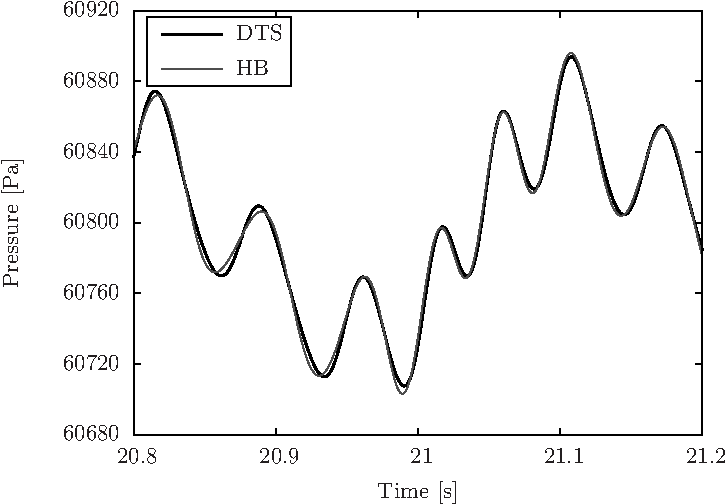
\includegraphics[width=.45\textwidth]{CANAL2_VALIDATION_HBT_GEAR_TIME_EV_PROBE_1.pdf}}
   \quad\subfigure[Probe
   2]{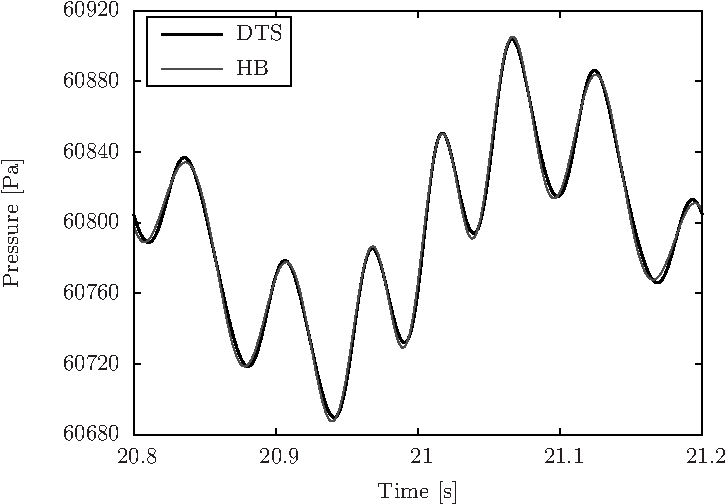
\includegraphics[width=.45\textwidth]{CANAL2_VALIDATION_HBT_GEAR_TIME_EV_PROBE_2.pdf}}
   \subfigure[Probe
   3]{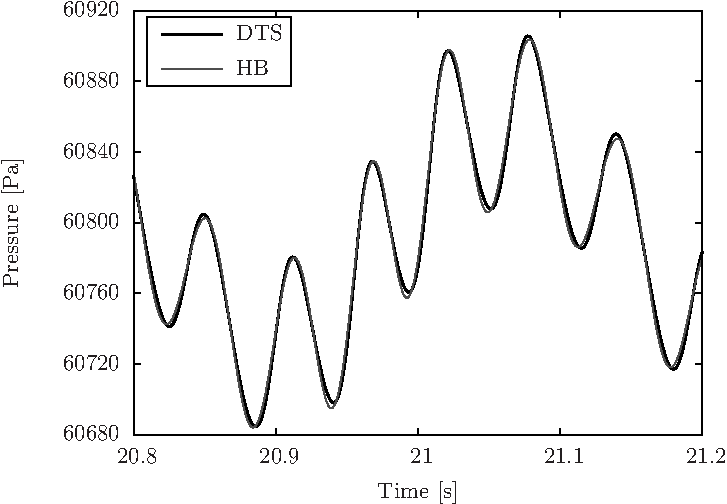
\includegraphics[width=.45\textwidth]{CANAL2_VALIDATION_HBT_GEAR_TIME_EV_PROBE_3.pdf}}
  \caption{Unsteady pressure signals at different axial positions.}
  \label{fig:canal2_validation_hbt_gear_time_ev}
\end{figure}

The goal of this section was not to show significant CPU savings but
rather the capacity of the present HB method to capture an
almost-periodic flow on a model problem.  It is now applied to a more
complex configuration, namely a turbomachinery element, where its
computational efficiency is also emphasized.






\section{Convection equation solver}




% chapter validation (end)